\documentclass[11pt,a4paper]{article}
\usepackage{fontspec}
\setmainfont{Cambria}
\setmonofont{Consolas}[Scale=0.9]
\usepackage[spanish,es-noshorthands,es-tabla]{babel}
\usepackage[margin=2.2cm]{geometry}
\usepackage{amsmath,amssymb}
\usepackage{booktabs,tabularx,array,longtable}
\usepackage{graphicx}
\usepackage{xcolor}
\usepackage{tikz}
\usetikzlibrary{arrows.meta,positioning}
\usepackage{enumitem}
\usepackage{caption}
\captionsetup{font=small,labelfont=bf}
\usepackage[hidelinks]{hyperref}
\usepackage{float}
\renewcommand{\arraystretch}{1.25}

\definecolor{caja}{HTML}{F2F1EC}
\newcommand{\enpalabras}[1]{%
  \par\smallskip\noindent\colorbox{caja}{\parbox{\dimexpr\linewidth-2\fboxsep}{\small\textbf{En palabras.} #1}}\par\smallskip}

\title{\textbf{Sistema de condición invernal para caminos de alta montaña}\\[4pt]
\large Índice de severidad andino, peligro, balance de despeje y estados operacionales}
\author{Catastro FONDEF -- Parte 2 (condición invernal de caminos de montaña)}
\date{Versión 2 · 12 de octubre de 2026}

\begin{document}
\maketitle

% ============================================================================
\section*{Resumen en una página}

\textbf{El punto de partida.} El protocolo de Lo Barnechea (3 de julio de 2026) funciona: ordena la decisión en tres alertas con umbrales concretos de nieve, isoterma, lluvia, visibilidad y tránsito. Pero resume todo en un solo número y por eso solo distingue entre abierto, cierre parcial y cierre total. No dice cuánto dura un cierre, no separa la tormenta del peligro posterior y no conecta la decisión con la maquinaria disponible.

\textbf{La propuesta.} Un sistema de cuatro piezas, calculado por tramo y cada 6 horas: un índice de severidad, un índice de peligro, un balance de despeje y una máquina de seis estados. La severidad sigue el método de Walker, pero con la isoterma convertida en fracción del camino bajo nieve y con el protocolo de Lo Barnechea como piso. El peligro va aparte: sube después de la tormenta y se resuelve esperando, no despejando. El balance lleva la cuenta de la nieve por sacar con la maquinaria disponible. Los estados se recorren en orden: se entra a un cierre por magnitud y se sale por fase. Lo que no depende del clima (horario fronterizo, decisión binacional, tránsito, condición sanitaria) queda en una capa aparte.

\textbf{Lo que muestran julio y agosto de 2026.} El sistema se calibró con la G-21 y se probó en la 60-CH. En la G-21 funciona: reproduce el estado observado con kappa ponderado de 0,54, contra 0,27 del cuadro del protocolo de Lo Barnechea, y clasifica como cierre por peligro 10 de los 11 bloques del corte del 17 al 20 de julio sin ver el estado observado. Pero lo hace por el peligro de avalancha del tramo alto, mientras que el corte se decretó por rodados, nieve y un aluvión del río Ñilhue en el tramo medio, que el índice de remoción en masa no detectó. La regla de Walker pura se ajusta mejor a la práctica (0,63), porque el piso del protocolo de Lo Barnechea manda a Alerta 2 la ``presencia de lluvia'' con isoterma alta y exige cierre total con poco más de 1 cm de nieve cuando la isoterma baja de 1.500 m, y la práctica no hace ninguna de las dos cosas. El peligro, en cambio, tiene que ir aparte: metido como una variable más, el sistema cierra la 60-CH en 1 de sus 176 bloques cerrados.

\textbf{El cierre largo de la 60-CH.} De los 36 días cerrados entre el 14 de julio y el 18 de agosto, el sistema respalda cierre total en 20, casi todos por peligro de avalancha. En los otros 16 justifica cierre parcial (3), restricción (9) o nada (4). Contando todo el periodo, entre el 41\,\% y el 58\,\% de las 1.019 horas cerradas no tienen respaldo meteorológico para cierre total, según la capacidad de despeje. Esto no prueba que la decisión haya sido errada. Primero, el resultado depende de la exposición del tramo alto a avalanchas, que hoy es un supuesto. Segundo, el sistema no ve la visibilidad: del 5 al 8 de agosto hubo ráfagas de hasta 31 m/s. Lo que sí muestra es que había opciones intermedias, y qué dato falta para elegir entre ellas: un catastro de trayectorias de avalancha.


\textbf{Cómo leer el documento.} La sección~\ref{sec:contexto} presenta las rutas, los datos y el protocolo de Lo Barnechea. La sección~\ref{sec:partida} dice de dónde sale cada pieza y por qué ni el protocolo de Lo Barnechea ni el índice de Walker bastan por sí solos. Las secciones~\ref{sec:arquitectura} a~\ref{sec:administrativa} formulan el sistema; cada fórmula va precedida de un recuadro ``en palabras''. Las secciones~\ref{sec:calibracion} y~\ref{sec:contrafactual} lo prueban con julio y agosto de 2026. La~\ref{sec:operacion} explica cómo se opera con pronóstico y en rutas sin protocolo; la~\ref{sec:limites}, lo que todavía no puede hacer.

\newpage
% ============================================================================
\section{Contexto: rutas, datos y el protocolo de Lo Barnechea}\label{sec:contexto}

\enpalabras{Dos caminos de alta montaña de Chile central, dos meses de invierno y una regla escrita. La G-21 sube de Lo Barnechea a Farellones y a los centros de esquí; la 60-CH sube de Los Andes al paso internacional Los Libertadores. Las dos se cerraron por nieve en julio y agosto de 2026. La primera se gobierna por el protocolo de Lo Barnechea; la segunda, por decisiones binacionales con Argentina. Aquí el cuadro del protocolo de Lo Barnechea se aplica a las dos, como regla de referencia.}

\paragraph{Las rutas y sus tramos.} Cada ruta se divide en un tramo alto y uno medio, porque la nieve y la isoterma no tratan igual a los 1.000 que a los 3.000 metros (cuadro~\ref{tab:tramos}). La G-21 incluye los accesos G-251 y G-249, que el protocolo de Lo Barnechea cubre junto con ella: unos 47 km de camino con más de 60 curvas y calzada de hasta 7 m. El tramo alto de la 60-CH va de Guardia Vieja al túnel del Cristo Redentor, pasando por Juncal y Portillo.

\begin{table}[H]
\centering\footnotesize\setlength{\tabcolsep}{4pt}
\caption{Tramos analizados. Largo de camino y cotas mínima, media y máxima (m s.\,n.\,m.) según el modelo digital de elevación Copernicus.}
\label{tab:tramos}
\begin{tabular}{|l|l|l|r|r|r|r|}
\hline
Ruta & Tramo & Recorrido & Largo (km) & Mín. & Media & Máx. \\ \hline
60-CH & alto & Guardia Vieja -- túnel Cristo Redentor & 28,9 & 1.644 & 2.431 & 3.700 \\ \hline
60-CH & medio & Río Blanco -- Guardia Vieja & 23,7 & 1.021 & 1.289 & 1.645 \\ \hline
G-21 & alto & Farellones y accesos (G-21, G-249, G-251) & 20,8 & 2.330 & 2.615 & 3.027 \\ \hline
G-21 & medio & subida de curvas desde Lo Barnechea & 29,6 & 917 & 1.507 & 2.463 \\ \hline
\end{tabular}
\end{table}

\paragraph{Los datos meteorológicos.} El análisis no usa estaciones meteorológicas. La meteorología sale de dos reanálisis del Centro Europeo (ECMWF): ERA5-Land, con celdas de unos 9 km, para nieve, lluvia, temperatura y manto; y ERA5, con celdas de unos 31 km, para la isoterma 0\,°C y las ráfagas de viento. Un reanálisis reconstruye, hora a hora, el tiempo que hubo: sirve para revisar lo que pasó, no para anticipar. Cada tramo promedia las celdas que cruza, ponderadas por el largo de camino dentro de cada una, en bloques de 6 horas locales del 1 de julio al 31 de agosto de 2026.

\paragraph{El estado observado.} Para cada hora del periodo, el equipo reconstruyó el estado de cada ruta a partir de comunicados y declaraciones oficiales de cierre y apertura, en cinco categorías: abierto; restringido (un solo sentido, solo carga, solo residentes y trabajadores, ventanas de evacuación o saturación); cierre técnico (pausa programada para despeje con máquinas); cierre meteorológico; y cierre por horario administrativo del complejo fronterizo.

\paragraph{El cuadro del protocolo de Lo Barnechea.} La sección 6 del protocolo de Lo Barnechea define tres alertas. Basta un gatillante para activar una alerta, y manda la más alta que se cumpla (cuadro~\ref{tab:cuadro}). La sección 7 agrega que la Alerta 2 permite cerrar la subida y mantener la bajada, y que la Alerta 3 implica cierre total.

\begin{table}[H]
\centering\footnotesize\setlength{\tabcolsep}{4pt}
\caption{Gatillantes del protocolo de Lo Barnechea (sección 6), por alerta. Nieve y lluvia en ventanas de 12 horas; isoterma 0\,°C en m s.\,n.\,m.}
\label{tab:cuadro}
\begin{tabularx}{\textwidth}{|>{\raggedright\arraybackslash}p{1.9cm}|>{\raggedright\arraybackslash}X|>{\raggedright\arraybackslash}X|>{\raggedright\arraybackslash}X|}
\hline
Gatillante & Alerta 1 (preventiva) & Alerta 2 (cierre parcial: solo bajada) & Alerta 3 (cierre total) \\ \hline
Nieve & más de 1 y menos de 25 cm, con cualquier isoterma & más de 25 y menos de 50 cm, con isoterma entre 1.500 y 2.800 m & más de 1 y menos de 50 cm con isoterma entre 900 y 1.500 m; 50 cm o más con isoterma entre 1.501 y 2.800 m \\ \hline
Lluvia & -- & presencia de precipitación líquida & 20 mm o más con isoterma sobre 2.800 m \\ \hline
Visibilidad & más de 50 y hasta 100 m & más de 21 y hasta 50 m & 20 m o menos \\ \hline
Tránsito de subida (08:00--13:00) & más de 0 y menos de 3.500 vehículos/día & más de 3.500 vehículos/día & -- \\ \hline
Condición sanitaria & -- & -- & falla de agua o baños por más de 24 h \\ \hline
\end{tabularx}
\end{table}

\paragraph{El cuadro regularizado.} El cuadro deja combinaciones sin alerta: por ejemplo, 30 cm con isoterma bajo 1.500 m, o 60 cm con isoterma sobre 2.800 m. Para poder calcularlo en cada bloque, este trabajo lo completa por bandas de isoterma, de modo que más nieve nunca baje la alerta. Con isoterma bajo 1.500 m, cualquier nevada sobre 1 cm es Alerta 3. Entre 1.500 y 2.800 m, los cortes son 1, 25 y 50 cm para las alertas 1, 2 y 3. Sobre 2.800 m, la nieve sobre 1 cm es Alerta 1, la lluvia de 1 mm o más es Alerta 2 y la de 20 mm o más es Alerta 3. Hay una diferencia con el cuadro literal: con isoterma bajo 2.800 m, la regularización no cuenta la ``presencia de precipitación líquida''. En el resto de las combinaciones que el cuadro define, el resultado es el mismo. La visibilidad, el tránsito y la condición sanitaria no están en los reanálisis y quedan fuera del cálculo.

% ============================================================================
\section{Punto de partida: qué es del protocolo de Lo Barnechea, qué de la literatura y qué es nuestro}\label{sec:partida}

\enpalabras{Ninguna pieza sale de la nada. El cuadro de niveles viene del protocolo de Lo Barnechea; las notas y los pesos, del índice de Walker; la capacidad de despeje, de la literatura canadiense; el umbral de arrastre, de la hidrología de nieve. Lo nuevo es el ensamblaje: la fracción del camino bajo nieve, el piso del protocolo de Lo Barnechea y dos estados que ese protocolo no tiene, ``despejando'' y ``en peligro''.}

\begin{table}[H]
\centering\small
\caption{Origen de cada elemento del sistema.}
\label{tab:origen}
\begin{tabularx}{\textwidth}{|>{\raggedright\arraybackslash}p{4.3cm}|>{\raggedright\arraybackslash}X|}
\hline
Elemento & Origen \\ \hline
Umbrales de nieve (1, 25 y 50 cm en 12 h), bandas de isoterma, lluvia 20 mm & Protocolo de Lo Barnechea, sección 6 \\ \hline
Notas 0--5 por variable y combinación con pesos & Walker, Anderson y Esmaeili (2018), índice de severidad invernal de Nebraska (NEWINS) \\ \hline
Fijar cortes con datos locales; no adoptar un índice ajeno & Sturges et al. (2020), Clear Roads CR 18-03; Walker et al. (2019) \\ \hline
Capacidad de despeje $c = d\,s/(p\,\ell)$ y plazos de recuperación & Muresan et al. (2018), cap. 13 \\ \hline
Pasadas según ancho de calzada; esfuerzo con clima en grilla & Mohammadi, Klein-Paste y Lysbakken (2024) \\ \hline
Umbral de arrastre $U^{\mathrm{thr}}(T)$ y nieve seca o húmeda & Li y Pomeroy (1997) \\ \hline
Criterio de nieve arrastrada (5 cm en 72 h) & Matthews et al., citado en Mohammadi y Klein-Paste (2023) \\ \hline
Estado post-tormenta con pronóstico de reapertura & Cerda et al. (2016), mina Andina (Andes centrales) \\ \hline
Separar cierre por daño y por peligro; la decisión es del jefe de operaciones & ASTRA (2014), Suiza \\ \hline
Lluvia acumulada de varios días en el corredor de la 60-CH & Mergili, Marchant y Moreiras (2015) \\ \hline
\textbf{Fracción del camino bajo nieve $\varphi$, regla híbrida con piso del protocolo de Lo Barnechea, índice de peligro, estados $E_4$ y $E_5$, capa administrativa, contrafactual} & \textbf{Propuesta de este documento} \\ \hline
\end{tabularx}
\end{table}

\paragraph{Qué es el índice de Walker.} Walker, Anderson y Esmaeili (2018) construyeron el índice de severidad invernal del Departamento de Transporte de Nebraska. Cada día con nieve recibe una nota de 1 a 6 en siete variables: nieve caída, tasa de nevada, viento, temperatura del aire, fracción del distrito afectada, duración y visibilidad. Las siete notas se promedian con pesos fijos (la nieve pesa 0,80; la visibilidad, 0,01) y dan la categoría del día. La suma de categorías de la temporada es el índice estacional, que sirve para comparar inviernos y evaluar el desempeño del mantenimiento.

\paragraph{Por qué no basta con recalibrar Walker.} Recalibrar Walker da un mejor termómetro, no un sistema de decisión. La salida simple sería tomar el índice de Nebraska, reemplazar sus cortes por cortes chilenos y aplicarlo tal cual. Eso corrige la escala: sin recalibrar, el techo de Walker (17,5 cm de nieve en 24 h) cae dentro de la Alerta 1 del protocolo de Lo Barnechea. Pero no corrige la forma, y la forma falla en cinco puntos.

\paragraph{Mide la tormenta, no el camino.} El índice de Walker clasifica días de nevada para comparar temporadas. No dice qué régimen operacional corresponde ni por cuánto tiempo. Un jefe de operaciones necesita ``cerrar la subida hasta que se despeje'', no ``categoría 5''.

\paragraph{Promedia lo que debería vetar.} Siete notas con pesos fijos, y la nieve se lleva el 80\,\%. Una condición extrema que no sea nieve apenas mueve la categoría: la visibilidad pesa 0,01, aunque el protocolo de Lo Barnechea cierra con visibilidad bajo 20 m sin mirar nada más. En nuestros datos, meter el peligro de avalancha dentro del promedio hace que el sistema nunca cierre la 60-CH (regla C, sección~\ref{sec:resultados}).

\paragraph{No tiene cota.} Walker se diseñó para la llanura de Nebraska. La temperatura entra porque la sal pierde efecto con el frío: más frío, más severo. En la cordillera el problema es otro: hasta qué cota llega la nieve y si llueve sobre el manto. Ahí una isoterma alta con lluvia puede ser peor que una nevada fría. Ninguno de los 19 índices de severidad que revisan Walker et al. (2019) usa la isoterma.

\paragraph{Termina cuando para de nevar.} El evento de Walker es el día con precipitación sólida. Lo que viene después (avalancha, calentamiento, lluvia sobre nieve, despeje) queda fuera. Un alud puede cortar el camino días después de la nevada; para el índice de Walker, ese día no existe.

\paragraph{No sabe de máquinas.} La categoría de Walker describe el impacto sobre el mantenimiento (``despliegue completo'', ``objetivo de servicio no se cumple''), pero no lo calcula. No conecta la severidad con la flota, el largo del tramo ni el tiempo de despeje, que es lo que decide cuándo reabrir.

\paragraph{Qué se toma de Walker.} El procedimiento: notas de 0 a 5 por variable, cortes fijados con datos locales y pesos explícitos. Es la pieza 1 del sistema. Las otras tres (peligro, despeje y estados) cubren lo que Walker no tiene.

\paragraph{Por qué no basta con el protocolo de Lo Barnechea.} El protocolo de Lo Barnechea dice cuándo cerrar, no cuándo abrir. Con los datos de julio y agosto de 2026, su cuadro casi nunca llega a la Alerta 3, y los cierres totales observados ocurrieron con 30 a 50 cm en 12 horas e isoterma entre 1.800 y 2.300 m: condiciones que el cuadro clasifica como Alerta 2. En la 60-CH, aplicado como referencia, el cuadro del tramo alto estuvo en Alerta 2 solo 5 de los 35 días que la ruta pasó cerrada, y nunca en Alerta 3. Nada en el cuadro indicaba cuándo reabrir.

% ============================================================================
% Formulación del sistema (secciones 2 a 7). Se incluye desde sistema_condicion_invernal.tex
% ============================================================================

\section{Arquitectura: cuatro piezas y una capa administrativa}\label{sec:arquitectura}

\enpalabras{El protocolo de Lo Barnechea responde con un solo número cuatro preguntas distintas: cuán dura es la tormenta, si hay peligro, cuánto falta para despejar y qué se hace con el tránsito. Por eso se queda en ``abierto'' o ``cerrado''. La propuesta separa esas preguntas en cuatro piezas encadenadas: la meteorología entra por arriba, pasa por la severidad, el peligro y el balance, y sale como un estado operacional con su hora estimada de reapertura.}

\begin{figure}[ht]
\centering
\begin{tikzpicture}[
  caja/.style={draw, rounded corners=3pt, align=center, minimum width=3.3cm, minimum height=1.25cm, font=\small, fill=gray!6},
  dato/.style={draw, dashed, rounded corners=3pt, align=center, minimum width=3.3cm, minimum height=1cm, font=\footnotesize},
  flecha/.style={-{Stealth[length=2.2mm]}, thick}]
\node[dato] (era) {ERA5 / ERA5-Land por tramo\\(o pronóstico GFS/ECMWF)};
\node[caja, below left=1.0cm and 1.2cm of era] (sv) {\textbf{1. Severidad} $SV$\\¿cuán dura es la tormenta?};
\node[caja, below right=1.0cm and 1.2cm of era] (h) {\textbf{2. Peligro} $H$\\avalancha y remoción};
\node[caja, below=2.9cm of era] (n) {\textbf{3. Balance de despeje} $N$\\¿cuánta nieve queda?};
\node[dato, right=0.7cm of n] (maq) {maquinaria, largo,\\ancho y pendiente};
\node[caja, below=1.0cm of n, minimum width=7cm] (e) {\textbf{4. Máquina de estados} $E_0,\dots,E_5$\\estado operacional y tiempo estimado de reapertura};
\node[dato, below=0.8cm of e, minimum width=7cm] (adm) {Capa administrativa (exógena): horario del complejo fronterizo,\\acuerdo binacional, tránsito, condición sanitaria};
\draw[flecha] (era) -- (sv); \draw[flecha] (era) -- (h); \draw[flecha] (era) -- (n);
\draw[flecha] (sv) |- (e); \draw[flecha] (h) |- (e);
\draw[flecha] (h) -- node[font=\footnotesize, right, pos=0.4]{$u_t$} (n);
\draw[flecha] (maq) -- (n); \draw[flecha] (n) -- (e);
\draw[flecha, dashed] (adm) -- (e);
\end{tikzpicture}
\caption{Arquitectura del sistema. Las flechas continuas son cálculos; la discontinua es una capa que se superpone al estado físico pero no se modela.}
\label{fig:arquitectura}
\end{figure}

\begin{table}[ht]
\centering\small
\caption{Qué pregunta responde cada pieza y qué tenía el protocolo de Lo Barnechea para esa pregunta.}
\label{tab:piezas}
\begin{tabularx}{\textwidth}{|>{\raggedright\arraybackslash}p{3.2cm}|>{\raggedright\arraybackslash}X|>{\raggedright\arraybackslash}X|}
\hline
Pieza & Pregunta & En el protocolo de Lo Barnechea \\ \hline
1. Severidad $SV$ & ¿Cuán dura es la tormenta en este tramo? & Nivel 1--3 por umbrales de nieve, isoterma y lluvia \\ \hline
2. Peligro $H$ & ¿Hay riesgo de avalancha o de remoción en masa, aunque ya no nieve? & ``Evaluación técnica'' sin criterio cuantitativo \\ \hline
3. Balance $N$ & ¿Cuánta nieve queda en la calzada y cuánto demora sacarla? & No existe; remite a un modelo municipal de limpieza aparte \\ \hline
4. Estados $E$ & ¿Qué régimen operacional corresponde y por cuánto tiempo? & Tres alertas, con cierre parcial (solo bajada) y total \\ \hline
Capa administrativa & ¿Hay razones no meteorológicas para cerrar? & Tránsito (3.500 veh/día), Waze, condición sanitaria \\ \hline
\end{tabularx}
\end{table}

\paragraph{Unidad de cálculo.} Todo se calcula por \textbf{tramo} $k$ (alto y medio de cada ruta) y por \textbf{bloque} $t$ de $\Delta = 6$ horas locales (00--06, 06--12, 12--18 y 18--24). La ventana de 12 horas del protocolo de Lo Barnechea son dos bloques.

\subsection*{Notación}
\begin{center}\small
\begin{tabular}{|>{$}l<{$}|l|l|}
\hline
\text{Símbolo} & Significado & Unidad \\ \hline
S_t & nieve caída en 12 h en las celdas ERA5-Land del tramo (agua equivalente $\times 10$) & cm \\ \hline
Z_t & altura de la isoterma 0\,°C & m s.\,n.\,m. \\ \hline
\varphi_t & fracción del largo del tramo bajo nieve & -- \\ \hline
S^*_t & nieve efectiva sobre el camino, $S^*_t = \varphi_t S_t$ & cm \\ \hline
r_t & tasa de nevada efectiva (nieve efectiva / horas con nieve) & cm/h \\ \hline
D_t & horas con nieve en las últimas 24 h & h \\ \hline
G_t & ráfaga máxima del bloque a 10 m (ERA5, \texttt{fg10}) & m/s \\ \hline
R_t & lluvia en 12 h cuando hay manto ($\ge 10$ cm) & mm \\ \hline
T_t & temperatura del aire a 2 m & °C \\ \hline
HN^{72}_t,\ R^{72}_t & nieve nueva y lluvia de las últimas 72 h & cm, mm \\ \hline
L_t & nivel del protocolo de Lo Barnechea (cuadro regularizado) & 0--3 \\ \hline
c_{i,t} & nota 0--5 de la variable $i$ & -- \\ \hline
SV_t,\ H_t & índices de severidad y de peligro & 0--5 \\ \hline
N_t & nieve por despejar en la calzada & cm \\ \hline
c_k,\ \theta & capacidad de despeje del tramo y nieve residual para reabrir & cm/h, cm \\ \hline
E_t & estado operacional & $E_0,\dots,E_5$ \\ \hline
\end{tabular}
\end{center}

% ----------------------------------------------------------------------------
\section{Pieza 1: índice de severidad andino}\label{sec:severidad}

\subsection{De la isoterma a la fracción del camino bajo nieve}

\enpalabras{En Nebraska, Walker mide qué parte del distrito está nevando. En la cordillera esa pregunta la responde la isoterma: hasta qué cota baja la nieve. Con isoterma baja nieva en todo el camino; con isoterma alta, solo en la parte de arriba. La fracción $\varphi$ mide cuánto del tramo queda sobre la línea de nieve y corrige la nieve de ERA5, que se calcula a la cota de la celda y no a la del camino. El protocolo de Lo Barnechea, en cambio, reparte la isoterma en tres bandas fijas y nunca pregunta ``¿cuánto camino quedó bajo nieve?''.}

La nieve no llega a la isoterma: cae unos cientos de metros más abajo. Con un margen $\delta$ (supuesto: $\delta = 300$ m), la fracción del tramo bajo nieve es
\begin{equation}
\varphi_t = \sum_{j \in k} \frac{\ell_j}{\ell_k}\; \min\!\left\{1,\ \max\!\left\{0,\ \frac{z^{\max}_j - (Z_t - \delta)}{z^{\max}_j - z^{\min}_j}\right\}\right\},
\label{eq:phi}
\end{equation}
donde $j$ recorre las celdas ERA5-Land que cruza el tramo, $\ell_j$ es el largo de camino dentro de la celda y $z^{\min}_j$, $z^{\max}_j$ son las cotas mínima y máxima del camino en ella (modelo digital de elevación Copernicus). Dentro de cada celda, la cota del camino se supone repartida de manera uniforme. La nieve efectiva sobre el camino es
\begin{equation}
S^*_t = \varphi_t\, S_t .
\end{equation}

\paragraph{Qué reemplaza $\varphi$.} Las tres bandas fijas del protocolo de Lo Barnechea (900--1.500, 1.500--2.800 y sobre 2.800 m). Así, una variable continua ocupa el lugar de tres categorías, y se calcula en cualquier ruta del catastro con su trazado y un modelo de elevación. Una isoterma baja da $\varphi \approx 1$: es el caso que ese protocolo trata como Alerta 3 (``nieve con isoterma entre 900 y 1.500 m'').

\subsection{Variables y notas de 0 a 5}

\enpalabras{Cada variable se convierte en una nota de 0 a 5: sube un punto por cada corte que supera. Los cortes de la nieve se anclan en los del protocolo de Lo Barnechea (1, 25 y 50 cm en 12 h); los intermedios siguen el procedimiento de Walker. La tasa, la duración y la extensión solo puntúan cuando hay evento de nieve (más de 1 cm en 12 h). El viento puntúa también cuando levanta nieve ya caída: ese protocolo no lo mira, aunque la ruta quede ``sin nevar, pero con viento blanco''.}

\begin{equation}
c_{i,t} = \sum_{j=1}^{5} \mathbf{1}\!\left[x_{i,t} \ge q_{i,j}\right], \qquad c_{i,t} \in \{0,1,\dots,5\},
\end{equation}
donde $x_{i,t}$ es el valor de la variable y $q_{i,1} < \dots < q_{i,5}$ sus cortes (cuadro~\ref{tab:cortes}).

\begin{table}[ht]
\centering\small
\caption{Cortes de las notas (una nota sube un punto por cada corte superado) y pesos tipo Walker. Las celdas en negrita son umbrales del protocolo de Lo Barnechea; el resto son propuestas de este documento.}
\label{tab:cortes}
\begin{tabular}{|l|l|c|c|c|c|c|c|}
\hline
Variable $i$ & Unidad & $q_1$ & $q_2$ & $q_3$ & $q_4$ & $q_5$ & Peso $\beta_i$ \\ \hline
Nieve efectiva 12 h, $S^*$ & cm & \textbf{1} & 10 & \textbf{25} & 40 & \textbf{50} & 0,45 \\ \hline
Fracción bajo nieve, $\varphi$ & -- & 0,05 & 0,25 & 0,50 & 0,75 & 0,95 & 0,15 \\ \hline
Tasa efectiva, $r$ & cm/h & 0,5 & 1 & 2 & 3 & 4 & 0,10 \\ \hline
Duración, $D$ & h en 24 h & 1 & 6 & 12 & 18 & 23 & 0,10 \\ \hline
Ráfaga, $G$ & m/s & 10 & 15 & 20 & 25 & 30 & 0,10 \\ \hline
Lluvia sobre manto, $R$ & mm en 12 h & \textbf{1} & 5 & 10 & \textbf{20} & 30 & 0,10 \\ \hline
\end{tabular}
\end{table}

\paragraph{Tres cambios respecto de Walker.} La nieve pesa 0,45, no 0,80: en la cordillera la extensión de la nevada y la lluvia sobre nieve tienen consecuencias propias que en Nebraska no existen. La temperatura del aire sale del índice: en Walker cuenta porque la sal pierde efecto con el frío, y aquí entra por dos vías más directas, la isoterma (vía $\varphi$) y el umbral de arrastre (pieza 3). El viento usa ráfagas de ERA5, no el viento medio de ERA5-Land: en nuestros tramos el viento medio tiene mediana cercana a 1 m/s y nunca alcanza un umbral de arrastre (sección~\ref{sec:resultados}).

\subsection{Tres reglas para combinar las notas}

\enpalabras{Walker promedia: una variable extrema pesa poco si no es la nieve. El protocolo de Lo Barnechea toma el máximo: basta un gatillante y manda el más alto. La regla híbrida combina las dos: el índice es el mayor entre el promedio de Walker y un piso que fija ese protocolo. Así nunca queda por debajo de lo que ya exige, pero distingue tormentas que su cuadro ve iguales: para el cuadro, ``26 cm con viento y nevando 20 horas'' es lo mismo que ``26 cm en calma''. El documento calcula también la regla de Walker pura, para que la elección sea informada.}

La suma ponderada es
\begin{equation}
W_t = \sum_{i} \beta_i\, c_{i,t}, \qquad \sum_i \beta_i = 1, \qquad 0 \le W_t \le 5 .
\end{equation}
El \textbf{piso} (veto) traduce el nivel del protocolo de Lo Barnechea $L_t$ a la escala 0--5:
\begin{equation}
v_t = v(L_t), \qquad v(0)=0,\quad v(1)=1,\quad v(2)=3,\quad v(3)=4 .
\end{equation}
$L_t$ sale del cuadro regularizado de la sección~\ref{sec:contexto}: el cuadro literal completado por bandas de isoterma, para que más nieve nunca baje la alerta. El cuadro se evalúa en cada hora, con la nieve y la lluvia de las 12 horas anteriores, y $L_t$ es el nivel horario más alto dentro del bloque: así se aplica en la práctica, de forma continua. Las dos reglas que se comparan son
\begin{align}
\text{(A) híbrida, propuesta:}\quad & SV^{A}_t = \max\{v_t,\ W_t\}, \label{eq:svA}\\
\text{(B) Walker pura:}\quad & SV^{B}_t = W_t . \label{eq:svB}
\end{align}

\paragraph{Monotonía.} Más nieve nunca baja el índice. Cada nota $c_{i,t}$ es no decreciente en su variable, los pesos son positivos y el cuadro regularizado es no decreciente en $S$ y en $R$; por lo tanto $W_t$, $v_t$ y $SV^A_t$ son no decrecientes en la nieve y en la lluvia. El cuadro literal del protocolo de Lo Barnechea no cumple esta propiedad: deja combinaciones sin nivel.

\paragraph{Piso.} La regla A es al menos tan exigente como el protocolo de Lo Barnechea, nunca menos. Como $SV^A_t \ge v_t$ y los umbrales de estado (sección~\ref{sec:estados}) están en $v(1)=1$, $v(2)=3$ y $v(3)=4$, toda situación que ese protocolo lleva a Alerta 1, 2 o 3 produce al menos restricción, cierre parcial o cierre total. La regla B no da esa garantía.

% ----------------------------------------------------------------------------
\section{Pieza 2: índice de peligro}\label{sec:peligro}

\enpalabras{El peligro corre por otro carril que la severidad. Sube \emph{después} de la tormenta, con calentamiento, con viento que carga las laderas o con lluvia sobre la nieve. Y no baja despejando: baja esperando, o con control de avalanchas. Por eso va en un índice propio, que decide dos cosas: si el camino se cierra por peligro y si las cuadrillas pueden entrar a trabajar. El protocolo de Lo Barnechea deja todo eso en una ``evaluación técnica'' sin criterio numérico.}

\subsection{Avalancha}
La nota de avalancha combina la nieve nueva de 72 horas en las zonas de partida (la celda ERA5-Land, más alta que el camino), el arrastre por viento y el calentamiento o la lluvia sobre un manto de al menos 30 cm:
\begin{equation}
H^{av}_t = \operatorname{red}\!\Big( e_k \cdot \min\big\{5,\ c^{HN}_t + a^{24}_t + \mathbf{1}[\Delta Z^{24}_t \ge 500 \ \lor\ R^{12}_t \ge 5]\cdot\mathbf{1}[h_t \ge 0{,}3]\big\}\Big),
\end{equation}
con $c^{HN}_t$ la nota de $HN^{72}_t$ (cortes 10, 20, 30, 50 y 80 cm), $a^{24}_t$ igual a 1 si hubo arrastre en las últimas 24 h, $\Delta Z^{24}_t$ el alza de la isoterma en 24 h, $h_t$ el espesor del manto y $e_k$ un factor de exposición del tramo (supuesto: 1 en los tramos altos y 0,5 en los medios, a falta de un catastro de trayectorias de avalancha). Las dos sobrecargas (arrastre, y calentamiento o lluvia) solo cuentan si $HN^{72}_t \ge 30$ cm: el viento y el calor son críticos sobre nieve reciente, no sobre un manto asentado.

\subsection{Remoción en masa}
\begin{equation}
H^{rm}_t = c^{R72}_t \cdot \mathbf{1}\!\left[Z_t > \bar z_k\right],
\end{equation}
con $c^{R72}_t$ la nota de la lluvia de 72 h (cortes 10, 20, 40, 60 y 100 mm) y $\bar z_k$ la cota media del tramo.

\paragraph{Por qué 72 horas.} En Guardia Vieja, el 13 de agosto de 1987, un flujo de detritos obligó a reconstruir la ruta internacional (148 mm en el día, 309,5 mm en cinco días; Mergili et al., 2015). La ventana de 12 h del protocolo de Lo Barnechea no capta esa acumulación.

\subsection{Peligro total y su efecto}
\begin{equation}
H_t = \max\{H^{av}_t,\ H^{rm}_t\}, \qquad u_t = \mathbf{1}\!\left[H_t < H^{\star}\right].
\end{equation}
Con $H_t \ge H^\star$ el camino pasa a cierre por peligro (si no está ya en cierre por tormenta) y las cuadrillas no despejan ($u_t = 0$). El umbral $H^\star$ se calibra con la G-21 entre 3, 4 y 5; el resultado es $H^\star = 5$ (sección~\ref{sec:calibracion}).

\subsection{Alternativa: el peligro dentro de la severidad}\label{sec:peligro_dentro}
\enpalabras{El peligro también puede entrar como una variable más del índice, sin estado propio. Es más simple, pero junta en un número dos cosas que se resuelven distinto: la tormenta se despeja, el peligro se espera. Se calcula como tercera regla, para comparar.}
\begin{equation}
\text{(C)}\quad SV^{C}_t = \max\big\{v_t,\ 0{,}85\, W_t + 0{,}15\, H_t\big\},
\end{equation}
sin estado $E_5$ y sin interrumpir el despeje. La comparación está en la sección~\ref{sec:resultados}.

% ----------------------------------------------------------------------------
\section{Pieza 3: balance de despeje}\label{sec:balance}

\enpalabras{Esta pieza convierte el modelo en un sistema de mantenimiento. En cada bloque entra a la calzada la nieve que cae y la que trae el viento, y sale la que la maquinaria alcanza a despejar, si se puede trabajar. Lo que queda es la nieve por despejar. Cuando baja del umbral, el camino se puede reabrir. La duración del cierre deja de ser una constante: sale de la nieve, del peligro y de la maquinaria. El protocolo de Lo Barnechea, en cambio, deriva esa pregunta a ``un modelo paramétrico de limpieza'' que vive fuera del cuadro.}

\begin{equation}
N_t = \max\big\{0,\ N_{t-1} + S^{*,6h}_t + A_t - u_t\, c_k\, \Delta\big\},
\label{eq:balance}
\end{equation}
donde $S^{*,6h}_t$ es la nieve efectiva caída en el bloque, $A_t$ la nieve redepositada por el viento y $c_k$ la capacidad de despeje del tramo.

\subsection{Capacidad de despeje en función de la maquinaria}
Una máquina que recorre un tramo de largo $\ell_k$ en $p_k$ pasadas a velocidad $s$ tarda $C = p_k \ell_k / s$ en completar un ciclo, y mantiene la calzada bajo una profundidad $d$ mientras la nieve no caiga más rápido que $d/C$ (Muresan et al., 2018, ec. 13.2--13.3). Con varias máquinas $m$:
\begin{equation}
c_k = \sum_{m \in \mathcal{M}_k} \frac{d\, s_m}{p_k\, \ell_k} .
\label{eq:capacidad}
\end{equation}
El número de pasadas sale del ancho de calzada, como en Noruega (Mohammadi et al., 2024): bajo 6 m, una pasada por sentido; entre 6 y 16 m, dos.

\paragraph{El dato que falta.} La velocidad de avance en nieve $s_m$ de cada tipo de equipo (cargador frontal, fresadora, bulldozer) no está en el inventario de maquinaria; hay que pedirla a Vialidad. Mientras tanto, $c_k$ se calibra con los cierres observados de la G-21 (sección~\ref{sec:calibracion}) y la ecuación~\eqref{eq:capacidad} se usa al revés, para traducir capacidades a flotas.

\subsection{Arrastre por viento}
Li y Pomeroy (1997, ec. 3) estiman el viento a 10 m que inicia el transporte de nieve seca, en función de la temperatura a 2 m:
\begin{equation}
U^{\mathrm{thr}}_t = 9{,}43 + 0{,}18\, T_t + 0{,}0033\, T_t^2 \quad [\text{m/s}].
\end{equation}
La relación se ajustó con viento medio horario y aquí se usan ráfagas, así que el umbral se escala por un factor de ráfaga $\gamma$ (supuesto: $\gamma = 1{,}6$). Hay arrastre cuando
\begin{equation}
a_t = \mathbf{1}\big[G_t \ge \gamma\, U^{\mathrm{thr}}_t\big] \cdot \mathbf{1}\big[\text{nieve seca}\big] \cdot \mathbf{1}\big[HN^{*,72}_t \ge 5\ \text{cm}\big],
\end{equation}
donde ``nieve seca'' significa que en las últimas 24 h la temperatura no llegó a 0\,°C y no llovió (definición de Li y Pomeroy, 1997), y los 5 cm en 72 h son el criterio de Matthews citado por Mohammadi y Klein-Paste (2023). La nieve redepositada es una fracción de la nieve reciente: $A_t = \alpha\, HN^{*,72}_t\, a_t$ (supuesto: $\alpha = 0{,}10$ por bloque).

\subsection{Tiempo de reapertura y flota necesaria}
\enpalabras{Del balance salen dos números que hoy nadie calcula: cuántas horas faltan para reabrir y cuántas máquinas harían falta para reabrir en un plazo dado. La pregunta deja de ser ``¿abrimos o no?'' y pasa a ser ``¿a qué hora, y con cuántos equipos?''.}
\begin{equation}
\widehat{T}^{\mathrm{reap}}_t = T^{\mathrm{espera}}_t + \frac{\max\{N_t - \theta,\ 0\}}{c_k},
\qquad
x^{\mathrm{req}} = \left\lceil \frac{(N_t - \theta)\, p_k\, \ell_k}{d\, \bar s\ T^{\mathrm{obj}}} \right\rceil ,
\end{equation}
donde $T^{\mathrm{espera}}_t$ es el tiempo hasta que el peligro baje de $H^\star$ (cero si ya está bajo) y $T^{\mathrm{obj}}$ el plazo objetivo.

\paragraph{Qué plazo pedir.} Hay una referencia publicada (Muresan et al., 2018, tabla 13.2): Ontario exige recuperar la calzada en 8, 16 o 24 h según la clase de camino, en el 90\,\% de los eventos.

% ----------------------------------------------------------------------------
\section{Pieza 4: máquina de estados}\label{sec:estados}

\enpalabras{El camino está siempre en uno de seis estados. Se entra a un cierre por la magnitud de la tormenta o del peligro, y se sale por fase: cuando deja de nevar, el cierre por tormenta pasa a cierre técnico, que dura lo que tarde la maquinaria en bajar la nieve bajo el umbral. Esta es la diferencia de fondo con el protocolo de Lo Barnechea, que no distingue entre ``está nevando'' y ``ya paró, pero falta despejar''.}

\begin{table}[ht]
\centering\small
\caption{Estados operacionales. La correspondencia con el protocolo de Lo Barnechea y con lo observado está en las dos últimas columnas.}
\label{tab:estados}
\begin{tabularx}{\textwidth}{|c|>{\raggedright\arraybackslash}p{3.3cm}|>{\raggedright\arraybackslash}X|>{\raggedright\arraybackslash}p{2.6cm}|>{\raggedright\arraybackslash}p{2.6cm}|}
\hline
Estado & Nombre & Qué implica & Protocolo de Lo Barnechea & Observado \\ \hline
$E_0$ & Abierto & Operación normal & Sin alerta & abierto \\ \hline
$E_1$ & Abierto con restricción & Cadenas, horarios, convoy & Alerta 1 & abierto o restringido \\ \hline
$E_2$ & Cierre parcial & Solo bajada; suben emergencias y suministros & Alerta 2 & restringido \\ \hline
$E_3$ & Cierre total meteorológico & Cerrado mientras dura la tormenta & Alerta 3 & cerrado (meteo) \\ \hline
$E_4$ & Cierre técnico / despeje & Ya no nieva; trabajan las máquinas & no existe & cierre técnico o cerrado \\ \hline
$E_5$ & Cierre por peligro & Avalancha o remoción; cuadrillas fuera & ``evaluación técnica'' & cerrado (p.\,ej. alud) \\ \hline
\end{tabularx}
\end{table}

Las reglas de transición se evalúan en orden, en cada bloque:
\begin{equation}
E_t =
\begin{cases}
E_3 & \text{si } SV_t \ge 3{,}5,\\
E_5 & \text{si no, y } H_t \ge H^\star,\\
E_4 & \text{si no, y } E_{t-1} \in \{E_3, E_4, E_5\} \ \text{y}\ N_t > \theta,\\
E_2 & \text{si no, y } SV_t \ge 2{,}5,\\
E_1 & \text{si no, y } \big(SV_t \ge 1 \ \text{o}\ N_t > \theta_1\big),\\
E_0 & \text{en otro caso,}
\end{cases}
\label{eq:estados}
\end{equation}
con $\theta_1 = 5$ cm (nieve en calzada que ya exige cadenas, cerca del umbral suizo de despeje de 3--5 cm; ASTRA, 2014).

\begin{figure}[ht]
\centering
\begin{tikzpicture}[
  est/.style={draw, circle, minimum size=1.35cm, align=center, font=\small, fill=gray!6},
  f/.style={-{Stealth[length=2mm]}, thick}, lab/.style={font=\scriptsize, align=center}]
\node[est] (e0) at (0,0) {$E_0$\\abierto};
\node[est] (e1) at (3.3,0) {$E_1$\\restr.};
\node[est] (e2) at (6.6,0) {$E_2$\\parcial};
\node[est] (e3) at (9.9,0) {$E_3$\\tormenta};
\node[est] (e4) at (6.6,-3.3) {$E_4$\\despeje};
\node[est] (e5) at (9.9,-3.3) {$E_5$\\peligro};
\draw[f] (e0) -- node[lab, above]{$SV\ge1$} (e1);
\draw[f] (e1) -- node[lab, above]{$SV\ge2{,}5$} (e2);
\draw[f] (e2) -- node[lab, above]{$SV\ge3{,}5$} (e3);
\draw[f] (e3) -- node[lab, right]{$H\ge H^\star$} (e5);
\draw[f] (e3) -- node[lab, above left, pos=0.45]{deja de nevar\\y $N>\theta$} (e4);
\draw[f] (e5) -- node[lab, below=12pt]{$H<H^\star$ y $N>\theta$} (e4);
\draw[f] (e4) -- node[lab, below left, pos=0.5]{$N\le\theta$} (e1);
\draw[f, bend left=40] (e1) to node[lab, below=1pt]{$SV<1$ y $N\le\theta_1$} (e0);
\end{tikzpicture}
\caption{Transiciones principales. Se entra a los cierres por magnitud ($SV$ o $H$) y se sale por fase y balance ($N$).}
\label{fig:estados}
\end{figure}

\paragraph{Estado de la ruta.} El estado observado es de la ruta completa; el modelado, el del tramo en peor situación, con el orden de gravedad $E_0 < E_1 < E_2 < E_4 < E_3 < E_5$.

\paragraph{Duración.} La duración es un resultado, no un parámetro. Un cierre dura la suma de sus bloques en $E_3$, $E_4$ y $E_5$, y esa suma sale de la tormenta, del peligro y de la capacidad de despeje.

% ----------------------------------------------------------------------------
\section{Capa administrativa y datos que hoy no tenemos}\label{sec:administrativa}

\enpalabras{Hay cierres que no dependen del clima: el horario del complejo fronterizo, un acuerdo con Argentina, la saturación del tránsito o la falta de agua en Farellones. El protocolo de Lo Barnechea los mezcla con los gatillantes meteorológicos, de modo que ``nieva mucho'' y ``no hay agua arriba'' llevan al mismo cierre. Aquí van a una capa aparte: se superponen al estado físico, se registran por separado y no entran a la calibración.}

\paragraph{Horario y acuerdo binacional.} Los bloques observados como ``cerrado por horario'' en la 60-CH se excluyen de la verificación. La decisión binacional de mantener el paso cerrado no se modela: es lo que el contrafactual de la sección~\ref{sec:contrafactual} compara con la condición física.

\paragraph{Tránsito y congestión.} El protocolo de Lo Barnechea usa 3.500 vehículos/día entre 08:00 y 13:00 y velocidades Waze bajo 5 km/h por 2 horas. No hay esos datos para julio y agosto de 2026. Cuando existan, entran como gatillantes de $E_1$ o $E_2$, no del índice de severidad.

\paragraph{Condición sanitaria.} Falla de agua o baños por más de 24 h (Alerta 3). Es un gatillante del destino, no del camino.

\paragraph{Visibilidad.} Está en el protocolo de Lo Barnechea (100, 50 y 20 m) pero no en ERA5. Cuando haya observación o pronóstico, entra como veto adicional $v_t$, con los mismos umbrales.


% ============================================================================
% Resultados con julio y agosto de 2026 (secciones 8 y 9)
% Números de: modelo_sam/salidas/sistema/*.csv (script sistema_condicion.py)
% ============================================================================

\section{Calibración y verificación con julio y agosto de 2026}\label{sec:calibracion}\label{sec:resultados}

\subsection{Datos y criterio}
\enpalabras{La G-21 calibra; la 60-CH se evalúa. La G-21 tiene un protocolo municipal funcionando, y sus cierres reflejan una práctica que vale la pena reproducir. La 60-CH tiene un cierre binacional de 35 días que se quiere \emph{evaluar}. Si el modelo se calibrara con ella, aprendería ``así decide la autoridad'' en vez de ``así se comporta la cordillera''.}

\paragraph{Entradas.} ERA5-Land por tramo (nieve, lluvia, temperatura, manto), isoterma ERA5 y ráfagas ERA5 (\texttt{fg10}, 0,25°), agregadas en bloques de 6 h locales entre el 1 de julio y el 31 de agosto de 2026 (248 bloques por tramo).

\paragraph{Observado.} El estado de la ruta descrito en la sección~\ref{sec:contexto}, agrupado en tres clases: abierto; restringido o cierre técnico; cerrado por meteorología. Un bloque cuenta como cerrado si tuvo al menos una hora de cierre meteorológico. Los bloques ``cerrado por horario'' quedan fuera (capa administrativa).

\paragraph{El cuadro del protocolo de Lo Barnechea.} El cuadro se aplica de forma continua. Su nivel se calcula en cada hora con la nieve y la lluvia de las 12 horas anteriores y la isoterma media de esas horas, y el nivel del bloque es el más alto que alcanzó dentro de él. Ese nivel es también el piso de la regla híbrida.

\paragraph{Modelo en tres clases.} $E_0$ y $E_1$ cuentan como abierto (con o sin cadenas); $E_2$, como restricción fuerte o cierre parcial; $E_3$, $E_4$ y $E_5$, como cerrado.

\paragraph{Métricas.} Cinco números, cada uno con una pregunta. El kappa ponderado mide el acuerdo en las tres clases descontando el que daría el azar (1 es acuerdo perfecto; 0, el del azar) y castiga más confundir ``abierto'' con ``cerrado'' que con ``restricción''. Para la clase ``cerrado'': el POD dice qué fracción de los bloques cerrados detecta el modelo; el FAR, qué fracción de los cierres del modelo no ocurrió; el CSI, los aciertos sobre aciertos, falsas alarmas y omisiones; y el HSS, cuánto mejor que el azar acierta el modelo.

\subsection{Parámetros calibrados}
La calibración busca en una grilla la capacidad de despeje $c$ (0,5 a 8 cm/h), la nieve residual para reabrir $\theta$ (5 a 50 cm) y el umbral de peligro $H^\star$ (3, 4 o 5) que maximizan el kappa ponderado en la G-21 (cuadro~\ref{tab:calibracion}).

\begin{table}[H]
\centering\small
\caption{Parámetros calibrados con la G-21.}
\label{tab:calibracion}
\begin{tabular}{|l|c|l|}
\hline
Parámetro & Valor & Comentario \\ \hline
Umbral de peligro $H^\star$ & 5 & mejor kappa con 5 (0,54) que con 4 (0,45) o 3 (0,30) \\ \hline
Capacidad de despeje $c$ & 6 cm/h & cota inferior: el kappa sube hasta 6 cm/h y luego se aplana (fig.~\ref{fig:curva_c}) \\ \hline
Nieve residual para reabrir $\theta$ & 50 cm & con $c \ge 6$ el resultado casi no depende de $\theta$ \\ \hline
\end{tabular}
\end{table}

La G-21 acota la capacidad, no la fija. Bajo unos 4 cm/h el modelo mantiene cerrada la G-21 cuando en la realidad ya estaba abierta (kappa 0,46 con 2 cm/h); desde 6 cm/h el ajuste ya no mejora (0,54 con 6 y con 8 cm/h). Por eso el contrafactual de la sección~\ref{sec:contrafactual} se repite con tres capacidades.

\begin{figure}[H]
\centering
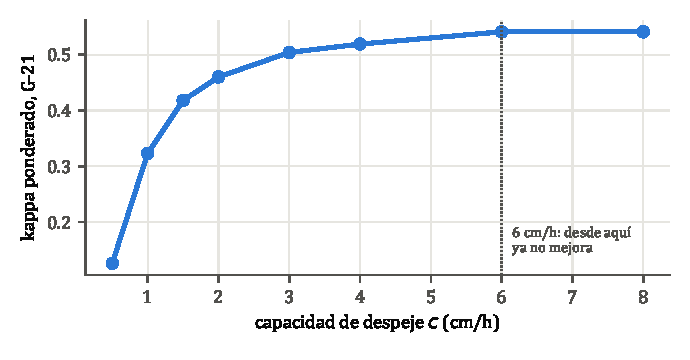
\includegraphics[width=0.62\textwidth]{fig/curva_capacidad.pdf}
\caption{Kappa ponderado de la G-21 según la capacidad de despeje. Con menos de unos 4 cm/h el modelo mantiene cerrada la G-21 cuando en la realidad ya estaba abierta; desde 6 cm/h el ajuste ya no mejora. La G-21 solo acota la capacidad por abajo.}
\label{fig:curva_c}
\end{figure}

\paragraph{Qué significa 6 cm/h en máquinas.} Con la ecuación~\eqref{eq:capacidad}, el tramo alto de la 60-CH ($\ell = 28{,}9$ km, $p = 2$ pasadas), una profundidad tolerada por pasada de $d = 10$ cm y una velocidad de avance de $s = 10$ km/h (valores ilustrativos, a confirmar con Vialidad), cada máquina aporta $c_1 = 10 \cdot 10 / (2 \cdot 28{,}9) \approx 1{,}7$ cm/h. Así, 6 cm/h equivalen a unas 3 o 4 máquinas trabajando a la vez en el tramo. El inventario de la 60-CH tiene 13 equipos activos de despeje: 4 cargadores frontales, 2 fresadoras de nieve, 5 bulldozers y 2 camiones con pala.

\subsection{Verificación: tres reglas y dos líneas base}

\begin{table}[H]
\centering\footnotesize\setlength{\tabcolsep}{4pt}
\caption{Verificación por bloque de 6 h. Kappa y exactitud en tres clases; POD, FAR, CSI y HSS para la clase ``cerrado''. G-21: 248 bloques, 19 cerrados. 60-CH: 212 bloques (sin los cerrados por horario), 176 cerrados. El cuadro del protocolo de Lo Barnechea usa solo sus gatillantes de nieve, lluvia e isoterma, con el nivel horario más alto de cada bloque; en la 60-CH se aplica como referencia, porque ese protocolo no rige ahí.}
\label{tab:metricas}
\begin{tabular}{|l|l|c|c|c|c|c|c|}
\hline
Modelo & Ruta & Exactitud & Kappa & POD & FAR & CSI & HSS \\ \hline
(A) Híbrida (propuesta) & G-21 & 0,79 & 0,54 & 0,68 & 0,46 & 0,43 & 0,57 \\ \hline
(A) Híbrida (propuesta) & 60-CH & 0,47 & 0,21 & 0,41 & 0,00 & 0,41 & 0,19 \\ \hline
(B) Walker pura & G-21 & 0,91 & 0,63 & 0,68 & 0,41 & 0,46 & 0,60 \\ \hline
(B) Walker pura & 60-CH & 0,47 & 0,17 & 0,41 & 0,00 & 0,41 & 0,19 \\ \hline
(C) Peligro dentro de la severidad & G-21 & 0,77 & 0,41 & 0,21 & 0,33 & 0,19 & 0,29 \\ \hline
(C) Peligro dentro de la severidad & 60-CH & 0,14 & 0,05 & 0,01 & 0,00 & 0,01 & 0,00 \\ \hline
Protocolo de Lo Barnechea (cuadro) & G-21 & 0,79 & 0,27 & 0,00 & 1,00 & 0,00 & $-$0,02 \\ \hline
Protocolo de Lo Barnechea (cuadro) & 60-CH & 0,14 & 0,04 & 0,01 & 0,00 & 0,01 & 0,00 \\ \hline
Persistencia (estado observado 6 h antes) & G-21 & 0,98 & 0,93 & 0,95 & 0,05 & 0,90 & 0,94 \\ \hline
Persistencia (estado observado 6 h antes) & 60-CH & 0,97 & 0,84 & 0,98 & 0,02 & 0,97 & 0,82 \\ \hline
\end{tabular}
\end{table}

\paragraph{El sistema frente al protocolo de Lo Barnechea.} El sistema ve los cierres que el cuadro no ve. Aplicado de forma continua, ese cuadro no detecta ningún cierre de la G-21 (POD 0) y da dos falsas alarmas, ambas el 8 de agosto. El sistema detecta 13 de los 19 bloques cerrados (kappa 0,54 contra 0,27).

\paragraph{El corte del 17 al 20 de julio.} El sistema justifica el corte, pero por otro mecanismo. La Resolución Exenta N.º 4.172 de la Dirección de Vialidad cortó la G-21 entre los kilómetros 1 y 36,3 por desprendimiento de rodados y acumulación de nieve; ese mismo día, un aluvión del río Ñilhue sobrepasó las mallas de contención entre los kilómetros 6 y 6,5. El sistema clasifica como cierre por peligro ($E_5$) 10 de los 11 bloques del corte, sin ver el estado observado, y la duración modelada se aparta de la observada en +1 y +7 horas (cuadro~\ref{tab:episodios}). Ese cierre, sin embargo, proviene del peligro de avalancha en el tramo alto (nota 5, con unos 35 cm de nieve en 12 h en la celda), mientras que el índice de remoción en masa del tramo medio, donde ocurrió el aluvión, no superó 2 de 5 (lluvia de 72 h de hasta 33 mm). El sistema no detectó el aluvión: el índice de remoción solo mira la lluvia de 72 horas y no ve la activación de quebradas.

\paragraph{El peligro aparte.} Diluido en un promedio, el peligro no pesa. Con la regla C el sistema cierra la 60-CH en 1 de sus 176 bloques cerrados y pierde la mayor parte de los cierres de la G-21 (POD 0,21). Separarlo no es una preferencia de diseño: es lo que permite justificar el cierre del 17 al 20 de julio.

\paragraph{Híbrida o Walker pura.} En la G-21 gana Walker pura, y la causa son dos reglas del protocolo de Lo Barnechea que entran por el piso (kappa 0,63 contra 0,54). Primero, en 34 bloques en que la G-21 estaba abierta, la híbrida marca cierre parcial porque el cuadro manda a Alerta 2 la ``presencia de precipitación líquida'' (50 de los 58 casos por tramo, todos con isoterma sobre 2.800 m). Segundo, el 8 de agosto la híbrida marca cierre total en dos bloques porque el cuadro exige Alerta 3 con más de 1 cm de nieve cuando la isoterma está entre 900 y 1.500 m: con 1,15 cm en 12 h e isoterma de 1.407 m, la G-21 estaba abierta. En la 60-CH la híbrida queda algo arriba (0,21 contra 0,17). La elección es de criterio. La híbrida garantiza cumplir ese protocolo; Walker pura se acerca más a lo que la práctica hace con la lluvia y con las nevadas mínimas. Hay una tercera vía: mantener la híbrida y revisar esas dos reglas en el cuadro de Lo Barnechea.

\paragraph{La persistencia.} La persistencia gana, pero juega otro partido. Repetir el estado de 6 horas antes acierta casi siempre (kappa 0,93 en la G-21), porque los estados duran muchos bloques. El sistema no mira el estado observado: todo sale de la meteorología. La persistencia sirve para el día a día, pero no dice si un cierre está justificado ni sirve en rutas sin historial.

\paragraph{La 60-CH.} En la 60-CH el bajo kappa es el resultado, no el error. Cuando el sistema cierra la 60-CH, el camino estaba cerrado (FAR 0). Lo que no reproduce es la duración: la mayor parte de las horas que la 60-CH estuvo cerrada, el sistema la considera transitable con restricción. La sección~\ref{sec:contrafactual} analiza esa diferencia.

\begin{figure}[p]
\centering
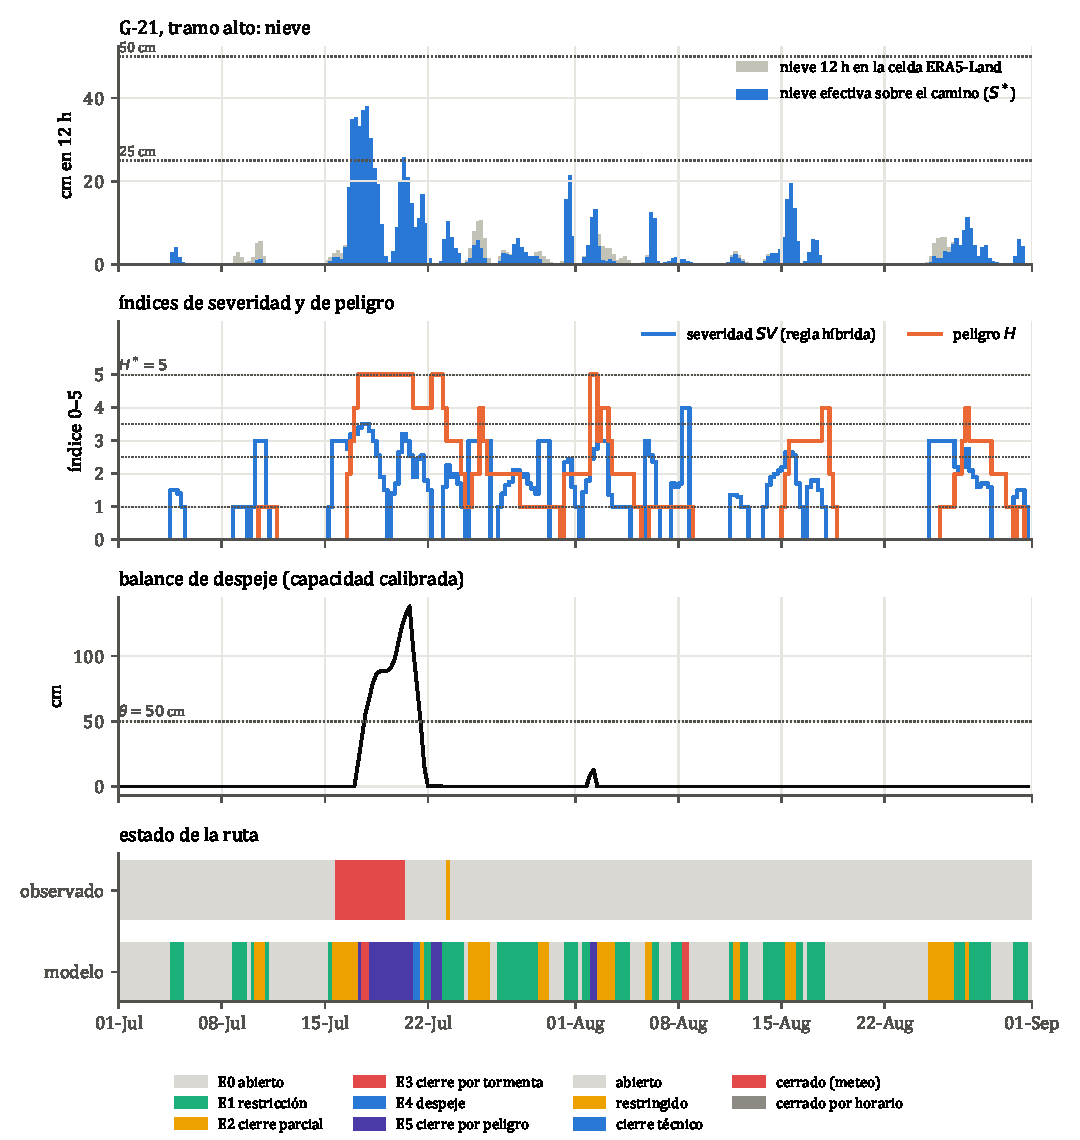
\includegraphics[width=\textwidth]{fig/serie_G21.pdf}
\caption{G-21, tramo alto. Arriba: nieve en 12 h en la celda ERA5-Land y nieve efectiva sobre el camino. Al medio: índices de severidad y de peligro, y balance de despeje. Abajo: estado observado de la ruta y estado del modelo (tramo en peor condición). El cierre de julio (tormenta, rodados y aluvión del río Ñilhue) cae en $E_3$ y $E_5$, con el peligro de avalancha del tramo alto; el resto del periodo el modelo marca sobre todo abierto o restricción.}
\label{fig:serieG21}
\end{figure}

\begin{table}[H]
\centering\footnotesize\setlength{\tabcolsep}{4pt}
\caption{Episodios de cierre meteorológico observados y lo que dice el modelo (capacidad calibrada). Bloques de 6 h en cada estado; ``h modelo'' son las horas que el modelo considera cerrado ($E_3$, $E_4$ o $E_5$).}
\label{tab:episodios}
\begin{tabular}{|l|l|r|r|r|r|r|r|r|r|}
\hline
Ruta & Episodio & h obs. & $E_0$ & $E_1$ & $E_2$ & $E_3$ & $E_4$ & $E_5$ & h modelo \\ \hline
G-21 & 15/07 23h -- 17/07 18h (lluvia y nieve) & 43 & 0 & 0 & 6 & 2 & 0 & 1 & 18 \\ \hline
G-21 & 17/07 18h -- 19/07 11h (rodados, nieve, aluvión) & 41 & 0 & 0 & 0 & 1 & 0 & 6 & 42 \\ \hline
G-21 & 19/07 17h -- 20/07 10h (rodados, nieve, aluvión) & 17 & 0 & 0 & 0 & 0 & 0 & 4 & 24 \\ \hline
60-CH & 09/07 17h -- 11/07 11h & 42 & 0 & 5 & 3 & 0 & 0 & 0 & 0 \\ \hline
60-CH & 14/07 15h -- 18/08 08h & 833 & 24 & 42 & 9 & 1 & 10 & 54 & 390 \\ \hline
60-CH & 24/08 17h -- 29/08 09h & 112 & 2 & 4 & 7 & 0 & 0 & 7 & 42 \\ \hline
60-CH & 29/08 17h -- 30/08 08h & 15 & 3 & 1 & 0 & 0 & 0 & 0 & 0 \\ \hline
60-CH & 30/08 17h -- 31/08 10h & 17 & 1 & 3 & 0 & 0 & 0 & 0 & 0 \\ \hline
\end{tabular}
\end{table}

\paragraph{Los episodios.} En la G-21 el sistema acierta el corte del 17 al 20 de julio, por peligro de avalancha y no por el aluvión, y se queda corto en el cierre preventivo. El cierre del 15 al 17 de julio se decretó por ``alarma de precipitaciones intensas'' (43 h); el sistema lo ve como cierre parcial casi todo el tiempo y solo cierra 18 h. En la 60-CH, el episodio del 9 al 11 de julio no tiene respaldo en ningún bloque: la isoterma media del 10 de julio estuvo en 3.280 m, así que la línea de nieve quedó cerca de los 3.000 m y la nevada apenas tocó el camino.

\subsection{Capa estadística: logit ordinal}
\enpalabras{Sobre las reglas cabe una capa estadística pequeña. Toma los tres números del sistema (severidad, peligro y nieve por despejar) y los convierte en probabilidades de ``abierto'', ``restricción'' o ``cerrado''. Se ajusta con la G-21. Aplicada a la 60-CH, responde qué habría decidido un operador que cerrara como se cierra la G-21.}

El modelo es un logit ordinal (de odds proporcionales):
\begin{equation}
P(Y_t \le j) = \frac{1}{1 + \exp\!\big(-(\alpha_j - \beta_{SV}\, \widetilde{SV}_t - \beta_H\, \widetilde{H}_t - \beta_N\, \widetilde{N}_t)\big)}, \qquad j \in \{0, 1\},
\end{equation}
con las variables estandarizadas, $Y_t$ la clase observada (0 abierto, 1 restricción, 2 cerrado) y una penalización ridge leve por los pocos cierres. Los coeficientes estandarizados ($\beta_{SV} = 1{,}31$, $\beta_H = 0{,}75$, $\beta_N = 0{,}55$) son los tres positivos, como se espera. En la G-21 alcanza kappa 0,57 (POD 0,53, FAR 0,29).

\paragraph{Qué significa en horas.} De las 1.019 horas que la 60-CH estuvo cerrada por meteorología, el criterio aprendido en la G-21 habría cerrado 288 (28\,\%). Así, un operador ``como el de la G-21'' habría mantenido la ruta abierta, con o sin restricción, las otras 731 horas. Probabilidad media de cierre en esas horas: 0,31.

% ============================================================================
\section{El cierre largo de la 60-CH: ¿había otras opciones?}\label{sec:contrafactual}

\enpalabras{La pregunta no es si la autoridad se equivocó. Es qué parte del cierre tiene respaldo en la condición física del camino. Para cada bloque cerrado, el sistema dice qué estado justifica la meteorología: ``cierre por tormenta'', ``por peligro'', ``despejando'', ``cierre parcial'', ``restricción'' o nada. La capacidad de despeje es incierta, así que el cálculo se repite con tres capacidades.}

\begin{figure}[H]
\centering
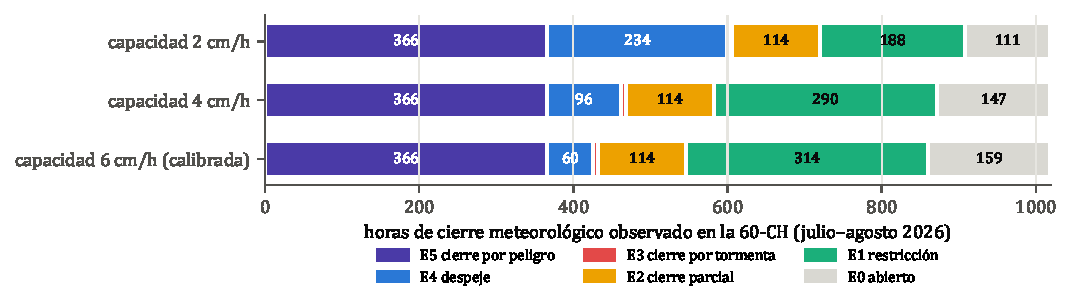
\includegraphics[width=\textwidth]{fig/contrafactual_60CH.pdf}
\caption{Las 1.019 horas de cierre meteorológico observado en la 60-CH (julio y agosto de 2026), según el estado que el sistema considera justificado, con tres capacidades de despeje. Las horas por peligro no dependen de la capacidad, porque con peligro alto no se despeja.}
\label{fig:contrafactual}
\end{figure}

\begin{table}[H]
\centering\footnotesize\setlength{\tabcolsep}{4pt}
\caption{Horas de cierre meteorológico observado en la 60-CH según el estado del modelo. ``Con respaldo'': el sistema justifica cierre total ($E_3$, $E_4$ o $E_5$). ``Sin respaldo'': justifica, como máximo, cierre parcial o restricción.}
\label{tab:contrafactual}
\begin{tabular}{|l|r|r|r|r|r|r|r|r|}
\hline
Capacidad & $E_5$ peligro & $E_3$ tormenta & $E_4$ despeje & $E_2$ parcial & $E_1$ restricción & $E_0$ abierto & Con respaldo & Sin respaldo \\ \hline
2 cm/h & 366 & 6 & 234 & 114 & 188 & 111 & 606 (59\,\%) & 413 (41\,\%) \\ \hline
4 cm/h & 366 & 6 & 96 & 114 & 290 & 147 & 468 (46\,\%) & 551 (54\,\%) \\ \hline
6 cm/h (calibrada) & 366 & 6 & 60 & 114 & 314 & 159 & 432 (42\,\%) & 587 (58\,\%) \\ \hline
\end{tabular}
\end{table}

\paragraph{La tormenta y el peligro.} La tormenta, por sí sola, casi nunca justificó cerrar la 60-CH; el peligro sí. Un solo bloque llega a $E_3$ (6 horas, el 17 de julio desde las 18:00), y lo hace por el piso del protocolo de Lo Barnechea: entre las 19:00 y las 22:00 la nieve de 12 h en la celda del tramo alto superó los 50 cm (hasta 51,6 cm), con isoterma cercana a 2.400 m, y el cuadro pasó a Alerta 3. En el resto, la nieve efectiva del tramo alto casi nunca supera los 40 cm en 12 h, porque la isoterma media diaria se mantuvo entre 2.100 y 3.600 m y solo una parte del camino quedó bajo nieve ($\varphi$ mediana de 0,38). Las 366 horas por peligro son las mismas con cualquier capacidad: con peligro alto no se despeja.

\paragraph{Día a día.} Entre el 14 de julio y el 18 de agosto (36 días, capacidad calibrada, estado más grave del día), el sistema da: 20 días con respaldo para cierre total, 19 por peligro de avalancha (16--23 y 25--30 de julio, 1--3 y 16--17 de agosto) y uno de despeje (24 de julio); 3 días de cierre parcial (15 de julio y 13--14 de agosto); 9 días de restricción con cadenas (31 de julio, 4--8, 11--12 y 15 de agosto); 4 días sin restricción meteorológica (14 de julio, 9--10 y 18 de agosto). Los días con respaldo coinciden con la gran tormenta de julio (unos 280 cm entre el 16 y el 21 en la celda ERA5-Land) y con las nevadas que siguieron sobre un manto que llegó a 2,3 m. El 14 de julio, el cierre se decretó con pronóstico, antes de que nevara.

\paragraph{La ventana del 4 al 12 de agosto.} Nueve días seguidos en que el sistema solo justifica restricción o apertura. Se leen en dos partes. Del 5 al 8 hubo poca nieve nueva (hasta 14 cm en 12 h en la celda, 9 cm efectivos), pero ráfagas de 25 a 31 m/s: viento blanco, que levanta la nieve y baja la visibilidad, un gatillante del protocolo de Lo Barnechea (Alerta 3 bajo 20 m) que ERA5 no entrega. Esos días pueden tener una justificación que el sistema no ve. Del 9 al 12, la nieve nueva de 72 h bajó a entre 3 y 15 cm, las ráfagas a entre 13 y 20 m/s, el peligro a 0 o 1 y el balance quedó en cero. Son los días con menos respaldo para el cierre total: el sistema indica que la ruta podía operar con restricción.

\paragraph{Qué se puede afirmar y qué no.} Con la calibración de la G-21, entre el 41\,\% y el 58\,\% de las horas de cierre de la 60-CH no tienen respaldo meteorológico para cierre total, según la capacidad de despeje. Un 11\,\% adicional justificaba solo cierre parcial. Esto no prueba que la decisión haya sido errada. Primero, el sistema no ve el lado argentino del paso, la visibilidad ni las evaluaciones de avalancha en terreno. Segundo, el resultado depende sobre todo de un supuesto: la exposición del tramo alto a avalanchas. Lo que sí muestra es que había opciones intermedias, que el protocolo de Lo Barnechea no contempla: cierre por peligro con ventanas de despeje, cierre parcial y restricción con cadenas. Y muestra qué dato falta para decidir mejor: un catastro de trayectorias de avalancha del tramo Juncal--Portillo--Los Libertadores.

\begin{figure}[p]
\centering
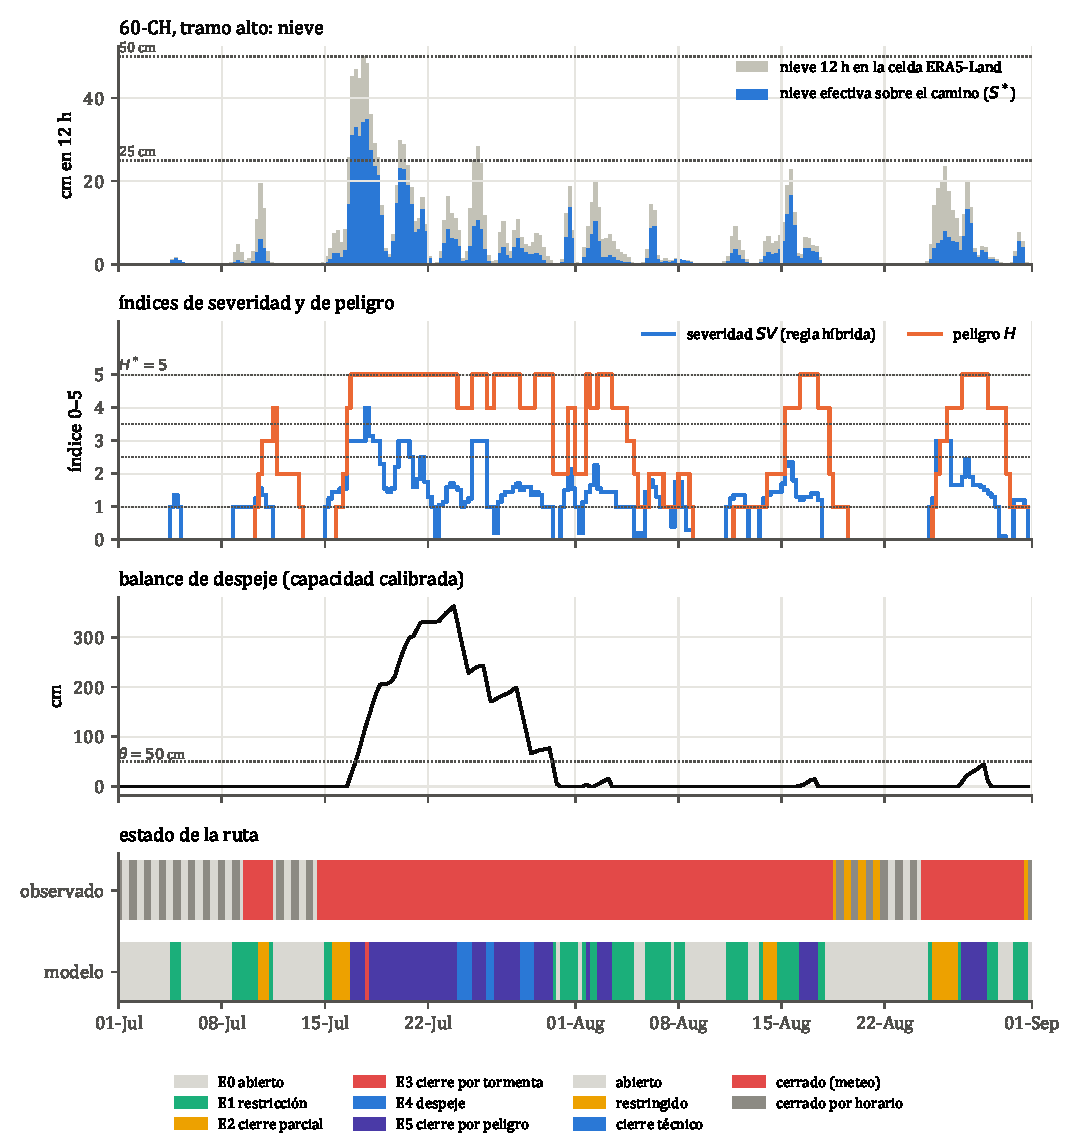
\includegraphics[width=\textwidth]{fig/serie_60CH.pdf}
\caption{60-CH, tramo alto, con la misma organización que la figura~\ref{fig:serieG21}. El cierre observado (rojo) se mantiene del 14 de julio al 18 de agosto. El modelo lo respalda con peligro ($E_5$) y despeje ($E_4$) hasta comienzos de agosto; luego pasa a restricción ($E_1$) y apertura ($E_0$), salvo un repunte de peligro el 16 y 17 de agosto. La nieve por despejar crece hasta unos 350 cm porque, con peligro alto, las cuadrillas no trabajan.}
\label{fig:serie60CH}
\end{figure}


% ============================================================================
\section{Cómo se usaría: pronóstico y rutas sin protocolo}\label{sec:operacion}

\subsection{Con pronóstico}
\enpalabras{En este documento el sistema corre con reanálisis: reconstruye lo que pasó. Sirve para calibrar y para revisar decisiones, no para operar. Para operar, corre con pronóstico y entra en los mismos plazos que ya fija el protocolo de Lo Barnechea: la reunión de D-7, la de D-3 y el día del evento. La diferencia es que en cada plazo sale, además del nivel de alerta, una hora estimada de reapertura.}

\paragraph{D-7.} Primera reunión de coordinación. Entra GFS o ECMWF por tramo, en tres escenarios (optimista, medio y pesimista, con los percentiles del conjunto). Salen los estados probables y las horas de despeje esperadas.

\paragraph{D-3.} Segunda reunión. Entra el pronóstico actualizado. Salen el estado esperado por bloque de 6 h, la hora estimada de reapertura y la flota necesaria $x^{\mathrm{req}}$ para cumplir un plazo objetivo.

\paragraph{D-0.} El día del evento, la observación reemplaza al pronóstico (estaciones, cámaras, reportes de ruta). El balance $N_t$ se reinicia con la nieve medida en la calzada.

\paragraph{Antes de operar.} Falta una prueba: repetir la verificación de la sección~\ref{sec:resultados} con pronósticos archivados y medir cuánto se degrada el sistema cuando el reanálisis se reemplaza por pronóstico.

\subsection{En rutas del catastro sin protocolo propio}
\enpalabras{Casi todo el catastro nacional no tiene protocolo ni historial de cierres. El sistema no los necesita: la nieve y la isoterma salen de ERA5, la fracción bajo nieve sale del trazado y un modelo de elevación, y la capacidad de despeje sale de la maquinaria de la provincia. Donde hoy solo hay ``la ruta se cierra cuando nieva mucho'', el sistema entrega estados, duraciones y flota.}

\paragraph{Qué se necesita por tramo.} Los cortes anclados al protocolo de Lo Barnechea (1, 25 y 50 cm) se mantienen; los intermedios salen de cuantiles de la climatología ERA5 del tramo, el mismo procedimiento de Walker. La fracción $\varphi$ sale del trazado del catastro de Vialidad y del modelo de elevación Copernicus. La capacidad $c_k$ sale de la ecuación~\eqref{eq:capacidad}, con la maquinaria asignada y el ancho de calzada. La exposición a avalanchas $e_k$ es hoy un supuesto (1 o 0,5); con un catastro de trayectorias se convierte en dato. Los parámetros pueden variar por tipo de ruta, como en California, Montana y Oregón, que usan coeficientes distintos para montaña, valle y llanura (Walker et al., 2019).

% ============================================================================
\section{Lo que el sistema no puede hacer todavía}\label{sec:limites}

\paragraph{Dos meses y dos rutas.} La calibración descansa en la G-21 de julio y agosto de 2026, con tres episodios de cierre meteorológico. Los parámetros describen esta temporada; lo transferible es la estructura.

\paragraph{Supuestos sin dato.} El margen de nieve bajo la isoterma ($\delta$), la exposición a avalanchas ($e_k$), el factor de ráfaga ($\gamma$), la fracción redepositada ($\alpha$), los pesos $\beta$ y los cortes intermedios son propuestas. El apéndice~\ref{sec:sensibilidad} mide cuánto mueve cada uno los resultados: solo la exposición los mueve de verdad.

\paragraph{La remoción en masa.} El índice de remoción solo mira la lluvia de 72 horas sobre la cota media del tramo. El 17 de julio de 2026, un aluvión del río Ñilhue sobrepasó las mallas de contención de la G-21 entre los kilómetros 6 y 6,5, y ese índice no pasó de 2 de 5 en el tramo medio. El cierre de esos días lo justificó el peligro de avalancha del tramo alto, no el aluvión. Para ver estos eventos falta un catastro de quebradas activas que cruzan cada ruta.

\paragraph{Los umbrales en el borde.} El cuadro del protocolo de Lo Barnechea tiene cortes duros, y el reanálisis los cruza por poco. El 17 de julio, la nieve de 12 horas en la celda del tramo alto de la 60-CH superó los 50 cm de la Alerta 3 durante cuatro horas, con un máximo de 51,6 cm. Un error de pocos centímetros en ERA5-Land cambia el nivel.

\paragraph{La velocidad de los equipos.} Sin la velocidad de avance en nieve de cada equipo, la capacidad de despeje se calibra en vez de calcularse. La fórmula de Muresan queda lista para cuando Vialidad entregue el dato.

\paragraph{Lo que ERA5 no ve.} Visibilidad, tránsito, estado de la calzada y el lado argentino del paso. ERA5-Land, además, puede sobrestimar la nieve en la alta cordillera: $\varphi$ corrige la cota, no el monto.

\paragraph{El contrafactual no juzga decisiones.} Mide qué parte de un cierre tiene respaldo meteorológico en el reanálisis, no si la decisión fue correcta. Una evaluación de avalanchas en terreno o una condición del lado argentino pueden justificar lo que el modelo no ve.

% ============================================================================
\begin{thebibliography}{99}\small
\bibitem{astra} Bundesamt für Strassen ASTRA (2014). \emph{Entscheidungsfindung und Auswertung bei Winterdiensteinsätzen}. Dokumentation ASTRA 86211, V1.00. Berna.
\bibitem{cerda} Cerda, P., Gallardo, L., Didier, M., Oyarzun Joaquin, M., Mujica Rodrigo y Vera Valero, C. (2016). Avalanche management in a large Chilean copper mine. \emph{Proceedings, International Snow Science Workshop 2016}, Breckenridge, 1348--1351.
\bibitem{li} Li, L. y Pomeroy, J. W. (1997). Estimates of threshold wind speeds for snow transport using meteorological data. \emph{Journal of Applied Meteorology}, 36, 205--213.
\bibitem{lob} Municipalidad de Lo Barnechea et al. (2026). \emph{Protocolo cierre de caminos públicos del Centro de Montaña Lo Barnechea}. 3 de julio de 2026.
\bibitem{mergili} Mergili, M., Marchant Santiago, C. I. y Moreiras, S. M. (2015). Causas, características e impacto de los procesos de remoción en masa, en áreas contrastantes de la región Andina. \emph{Cuadernos de Geografía}, 24(2), 113--131.
\bibitem{moh23} Mohammadi, N. y Klein-Paste, A. (2023). How to incorporate weather data in simulations of winter road maintenance? \emph{TRB 102nd Annual Meeting}.
\bibitem{moh24} Mohammadi, N., Klein-Paste, A. y Lysbakken, K. R. (2024). Simulating winter maintenance efforts: A multi-linear regression model. \emph{Cold Regions Science and Technology}, 227, 104307.
\bibitem{muresan} Muresan, M., Kwon, T. J., Fu, L. y Shi, X. (2018). Strategic planning and management for sustainable winter road maintenance. En X. Shi y L. Fu (Eds.), \emph{Sustainable Winter Road Operations} (cap. 13, 273--308). Wiley.
\bibitem{sturges} Sturges, L., Fay, L., Clouser, K. y Villwock-Witte, N. (2020). \emph{Evaluation of SSI and WSI Variables}. Clear Roads CR 18-03.
\bibitem{walker18} Walker, C., Anderson, M. y Esmaeili, B. (2018). \emph{Development of the Nebraska Department of Transportation Winter Severity Index}. NDOT SPR-P1-(17)M054.
\bibitem{walker19} Walker, C. L., Hasanzadeh, S., Esmaeili, B., Anderson, M. R. y Dao, B. (2019). Developing a winter severity index: A critical review. \emph{Cold Regions Science and Technology}, 160, 139--149.
\end{thebibliography}

\appendix
% ============================================================================
\section{Sensibilidad a los supuestos}\label{sec:sensibilidad}

\enpalabras{Cada supuesto sin dato se mueve por separado; el resto queda en su valor propuesto y los parámetros calibrados no cambian. Se mira qué pasa con el ajuste en la G-21 y con la parte del cierre de la 60-CH que queda sin respaldo. Un supuesto que ``mueve poco'' puede quedar como está; uno que ``lo mueve todo'' pide un dato.}

\begin{table}[H]
\centering\footnotesize\setlength{\tabcolsep}{4pt}
\caption{Sensibilidad. Kappa y CSI en la G-21; porcentaje de las horas cerradas de la 60-CH sin respaldo para cierre total y porcentaje respaldado por peligro (capacidad calibrada, 6 cm/h).}
\label{tab:sensibilidad}
\begin{tabular}{|l|c|c|c|c|}
\hline
Supuesto modificado & Kappa G-21 & CSI G-21 & 60-CH sin respaldo & 60-CH por peligro \\ \hline
Propuesta (base) & 0,54 & 0,43 & 58\,\% & 36\,\% \\ \hline
Margen de nieve $\delta$ = 150 m (base 300) & 0,54 & 0,43 & 59\,\% & 36\,\% \\ \hline
Margen de nieve $\delta$ = 500 m & 0,54 & 0,43 & 56\,\% & 35\,\% \\ \hline
Exposición de tramos medios = 1 (base 0,5) & 0,54 & 0,43 & 58\,\% & 37\,\% \\ \hline
Exposición de tramos altos = 0,75 (base 1) & 0,37 & 0,10 & 99\,\% & 0\,\% \\ \hline
Factor de ráfaga $\gamma$ = 2,0 (base 1,6) & 0,57 & 0,46 & 65\,\% & 29\,\% \\ \hline
Factor de ráfaga $\gamma$ = 1,3 & 0,50 & 0,39 & 56\,\% & 37\,\% \\ \hline
Sin nieve arrastrada ($\alpha$ = 0; base 0,10) & 0,54 & 0,43 & 61\,\% & 36\,\% \\ \hline
Sobrecargas desde 20 cm (base 30) & 0,54 & 0,43 & 58\,\% & 36\,\% \\ \hline
Sobrecargas desde 50 cm & 0,57 & 0,46 & 61\,\% & 32\,\% \\ \hline
Pesos de Walker (nieve 0,80; resto 0,04) & 0,55 & 0,43 & 58\,\% & 36\,\% \\ \hline
\end{tabular}
\end{table}

\paragraph{Lectura.} Un solo supuesto decide el resultado. El margen de nieve, los pesos y el umbral de las sobrecargas casi no mueven nada; el factor de ráfaga mueve algo (entre 56\,\% y 65\,\% sin respaldo). La exposición del tramo alto a avalanchas lo mueve todo: con 0,75 el peligro nunca llega a 5, desaparece el respaldo de los 19 días ``por peligro'' y la G-21 pierde el cierre por peligro del 17 al 20 de julio (kappa 0,37). Que el valor 1 reproduzca ese cierre apoya usarlo, aunque el corte real se decretó por rodados, nieve y un aluvión, no por una avalancha registrada. El dato correcto es un catastro de trayectorias de avalancha por tramo.

% ============================================================================
\section{Parámetros y reproducibilidad}\label{sec:parametros}

\begin{table}[H]
\centering\small
\caption{Parámetros del sistema. ``Calibrado'' = ajustado con la G-21; ``protocolo'' = tomado del protocolo de Lo Barnechea; ``literatura'' = con fuente; ``supuesto'' = propuesta a confirmar.}
\label{tab:parametros}
\begin{tabularx}{\textwidth}{|l|c|l|>{\raggedright\arraybackslash}X|}
\hline
Parámetro & Valor & Tipo & Nota \\ \hline
Umbrales de nieve en 12 h & 1, 25, 50 cm & protocolo & cortes $q_1$, $q_3$, $q_5$ de $S^*$ \\ \hline
Cortes intermedios y pesos $\beta$ & cuadro~\ref{tab:cortes} & supuesto & procedimiento de Walker; poco sensibles \\ \hline
Piso del protocolo de Lo Barnechea $v(L)$ & 0, 1, 3, 4 & propuesta & alinea Alerta 1, 2 y 3 con $E_1$, $E_2$ y $E_3$ \\ \hline
Umbrales de estado & 1; 2,5; 3,5 & propuesta & sobre $SV$ \\ \hline
Margen de nieve bajo la isoterma $\delta$ & 300 m & supuesto & poco sensible \\ \hline
Umbral de arrastre $U^{\mathrm{thr}}(T)$ & 9,43 + 0,18$T$ + 0,0033$T^2$ & literatura & Li y Pomeroy (1997), ec. 3 \\ \hline
Factor de ráfaga $\gamma$ & 1,6 & supuesto & moderadamente sensible \\ \hline
Nieve mínima para arrastre & 5 cm en 72 h & literatura & Matthews, en Mohammadi y Klein-Paste (2023) \\ \hline
Fracción redepositada $\alpha$ & 0,10 por bloque & supuesto & poco sensible \\ \hline
Sobrecargas del peligro & desde 30 cm en 72 h & supuesto & poco sensible \\ \hline
Exposición a avalanchas $e_k$ & 1 (alto), 0,5 (medio) & supuesto & \textbf{decisivo}; requiere catastro \\ \hline
Umbral de peligro $H^\star$ & 5 & calibrado & G-21 \\ \hline
Capacidad de despeje $c$ & 6 cm/h & calibrado & cota inferior; ec.~\eqref{eq:capacidad} para escenarios \\ \hline
Nieve residual para reabrir $\theta$ & 50 cm & calibrado & poco identificado \\ \hline
Nieve que exige restricción $\theta_1$ & 5 cm & literatura & cerca del umbral suizo de 3--5 cm (ASTRA, 2014) \\ \hline
\end{tabularx}
\end{table}

\paragraph{Reproducibilidad.} Todo el cálculo está programado y se repite con los mismos datos: la lectura de ERA5 y ERA5-Land por tramo, las cuatro piezas, la calibración con la G-21, la verificación, el logit ordinal, el contrafactual de la 60-CH, la sensibilidad y las figuras. Para cada tramo y bloque de 6 horas queda una tabla con las variables meteorológicas, las notas, los índices, el balance de despeje y el estado del modelo, junto al estado observado.


\end{document}
